\chapter{Ricorsione}
La programmazione ricorsiva è strettamente legata all'induzione matematica, si basa
sul fatto che per risolvere un problema mi riconduco a un problema non ancora risolto, 
ma più semplice, fino ad arrivare a un caso base già risolto.\\
I vantaggi della ricorsione sono due:
\begin{itemize}
    \item Più semplice rispetto agli algoritmi iterativi (solitamente)
    \item La logica ricorsiva è più efficiente rispetto a quella iterativa
\end{itemize}
\section{Fattoriale}
\subsection{Iterativo}
\begin{lstlisting}[language=Java]
    int Fatt(n)
        Ris=1
        For i=n downto 1
            Ris=Ris*i;
        return Ris;
\end{lstlisting}
\subsection{Ricorsivo}
\begin{lstlisting}
    int Fatt(int n)
        if n==0
            return(1);
        else
             Ris=(Fatt(n-1));
             Tot = n*Ris;
             return(Tot);
\end{lstlisting}
\section{Potenza ricorsiva}
\begin{lstlisting}{language=Java}
int Potenza (int A, int n)
c   if (n == 0)
c tif   return(1)
    else
NO c fif  Ris=A*Potenza(A, n-1)
NO c fif     return(Ris)
\end{lstlisting}
\subsection{Calcolo tempo di esecuzione}
In questo non avendo cicli dobbiamo controllare le funzioni ricorsive, è sbagliato
dire che la chiamata ricorsiva impiega $c*f_{if}$, perchè dipende da n non è un tempo
di esecuzione costante! Vedremo più avanti come calcolare il tempo di esecuzione.
\section{La ricorsione è sempre più efficiente rispetto all'iterazione?}
Prendiamo l'esempio della sequenza di Fibonacci eseguita ricorsivamente.
\begin{lstlisting}[language=Java]
int fibonacci(int n)
    if (n <= 1)
        return n;
    else 
        return fibonacci(n-1) + fibonacci(n-2);
\end{lstlisting}
Se scomponiamo l'esecuzione di questa funzione noteremo che vengono rieseguiti più volte
i calcoli per gli stessi numeri, dato che mi ritroverò più volte gli stessi numeri.
\begin{center}
    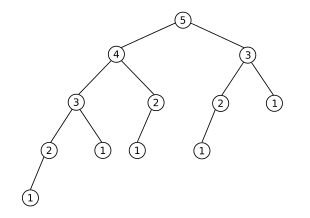
\includegraphics[width=50mm]{img/Fibonacci_Tree.png}
\end{center}
Notiamo infatti dall'albero che vengono calcolati più volte gli stessi numeri e questa
è una grande inefficienza.\\
In questi casi quindi l'iterazione risulta migliore rispetto alla ricorsione.
\section{Ricerca carattere in Array}
Dato un Array trova tutte le occorrenze di una lettera data in input (in questo caso z).\\
Devo sempre ricondurmi all'affermazione ricorsiva, quindi partire da un caso, ricondurmi
a uno più piccolo che però non mi da ancora il risultato, ma che mi avvicina sempre di più
al caso base.\\
In questo caso la penso nel seguente modo: Guarda A[n] se contiene z allora 1+tutte le z
in A[n-1] altrimenti 0 + tutte le z in A[n-1].\\
Fino a ricondurmi al primo elemento dell'array, il caso base sarà proprio quello! 
Controllare quando ho un solo elemento se è z o no, se è z ritorno 1 se no ritorno 0.
\subsection{Implementazione}
\begin{lstlisting}[language=Java]
    int trova(char car, char A[], int pos)
        if pos == 1
            if A[1] == 'z'
                return(1)
            else
                return(0)
        else
            Ris=trova(char car, char A[], pos -1)
            if A[pos] == 'z'
                Ris++
            return(Ris)
\end{lstlisting}
Solitamente nelle funzioni ricorsive per scorrere un array abbiamo bisogno di due indici,
per indicare la porzione di array che stiamo analizzando (es int h, int k), in questo
caso il primo indice è fisso dato che devo scorrere dall'ultimo valore a scendere fino al primo, quindi
sarebbe come avere h=1 fisso e k=k-1, quindi h non lo considero.\\
Le varie chiamate ricorsive mi portano a scorrere tutti i valori e quando mi riconduco al caso base, 
la risoluzione di tutte le chiamate aperte mi porta a controllare mano a mano tutti gli indici dell'array
restituendo mano a mano il contatore incrementato o meno a in base al fatto che ci sia z o meno.

\section{Divide et Impera}
Si tratta di un approccio di tipo ricorsivo che consiste in 3 fasi:
\begin{itemize}
    \item Problema P è diviso in due o più sottoproblemi - DIVIDE
    \item Ogni sottoproblema è risolto ricorsivamente - IMPERA
    \item Le soluzioni ai sottoproblemi sono riunite a formare la soluzione completa - COMBINA
\end{itemize}
\subsection{Ordinamento tramite Divide et Impera - Merge Sort}
Problema P, ordina un vettore A di n elementi (usando Divide et Impera):
\begin{itemize}
    \item Divide - Divido in 2 parti l'array da ordinare, ogni parto con $\frac{n}{2}$
    elementi, approssimando verso il basso nel caso il valore non fosse intero (n dispari)
    \item Impera - Ordina la prima metà, poi ordina la seconda metà
    \item Combina - Fonde (MERGE) in modo ordinato le due metà ordinate
\end{itemize}
\textbf{Merge sort è un algoritmo di ordinamento STABILE}.
\paragraph*{Definizione di algoritmo di ordinamento STABILE}
Un algoritmo di ordinamento si dice stabile se elementi di uguale valore al termine dell'ordinamento 
mantengono tra di loro l'ordine che avevano inizialmente.\\
Quindi se ho per esempio [1, 5, 3, 2a, 7, 0, 2b], una volta ordinato
avrò [0, 1, 2a, 2b, 3, 5, 7], i 2 anche se identici hanno preservato il loro ordina iniziale, quindi
2a si trova ancora prima di 2b.\\
Non è necessario che un algoritmo di ordinamento sia stabile per poter funzionare, ma questa 
caratteristica può essere utile per determinati utilizzi (strutture dati).
\subsection{Esecuzione ordinamento}
Dato che è necessario disegnare e usare diversi colori la spiegazione viene
riportata scritta a mano, qui di seguito il link per la visualizzazione.
\paragraph*{Note importanti} Nel libro sembra che l'esecuzione dei sottopassi sia effettata in maniera
parallela, NON è così, viene ordinata prima la prima metà, poi le sotto metà della prima, fino ad arrivare ai casi base,
poi si torna indietro a ritroso, non si ordinano parallelamente tutti i sotto array.\\
Nella spiegazione infatti gli ordinamenti sono stati messi a livelli di altezza diversi per sottolineare
questo aspetto.\\
Ecco il PDF \href{https://drive.google.com/file/d/1Ne8wRM-v0vQZlO_I1bBfiiJK-7Co7vqX/view?usp=sharing}{Link al PDF}.
\subsection{Implementazione codice}
\begin{lstlisting}
void MergeSort (A[], int pin, int pfin)
    if pin < pfin
        m = (pin + pfin) DIV 2 //DIVIDE
        //divisione intera approssima verso il basso
        MergeSort(A[], pin, m) //IMPERA
        MergeSort(A[], n+1, pfin) //IMPERA
        Merge(A[], pin, m, pfin) //COMBINA

B[] //Array di appoggio per Merge

void Merge(A[],In, meta, fin2)
    I1=In
    I2=meta+1
    Ib=In
    while I1 <= meta AND I2 <= fine
        if A[I1]<=A[I2] //Maggiore uguale rende Merge stabile
            B[Ib] = A[I1]
            IB++
            I1++
        else
            B[Ib] = A[I2]
            IB++
            I2++
    while I1 <= meta
        B[Ib] = A[I1]
        Ib++
        I1++
    while I2 <= fine
        B[Ib] = A[I2]
        Ib++
        I2++
    Ib=In
    while Ib <= fine //ricopio l'array ordinato nell'array iniziale
        A[Ib]=B[Ib]
        Ib++
\end{lstlisting}
\begin{itemize}
    \item pin e pfin sono rispettivamente l'indice iniziale e finale dell'array che sto analizzano
    (serve per dividere l'array per la divide)
    \item Li sommo e divido per 2 (divisione intera) per dividere l'Array e poi do in input la pin e la metà
    a una chiamata ricorsiva di MergeSort - DIVIDE
    \item Chiamo una funzione Merge (diversa da MergeSort) che ordina i sottoarray
\end{itemize}
\paragraph*{Merge}
\begin{itemize}
    \item Qua è come inserire indice inizio1, fine1, inizio2, fine2, ma dato che fine1 è la
     metà dell'array, e inizio2 e m+1, passo solo meta come parametro, ma il ragionamento in realtà è quello di passare
     gli indici di inizio e fine di 2 array
    \item if A[I1] $\leq$ A[I2] rende Merge stabile perchè se sono uguali scelgo di ordinare prima A[I1] quindi l'elemento
    di sinistra, questo mantiene i due elementi com'erano ordinati inizialmente
    \item Dopo il primo while aggiungo 2 while perchè potrebbe essere che la prima parte è ordinata e ho finito gli
    elementi, ma nella seconda ci siano ancora elementi, servono quindi a continuare a copiare gli elementi rimasti
    in una delle due parti quando l'altra parte è già stata ordinata. Chiaramente verrà eseguito uno dei due while, mai tutti
    e due.
    \item Ultimo while serve a ricopiare tutto nell'array iniziale A (copia B in A)
    \item Quest'ultimo ciclo while in realtà è un for perchè la dimensione dell'array da copiare è fissa, so già
    quante istruzioni devo eseguire
\end{itemize}
\paragraph*{Osservazione, perchè uso B e non lavoro direttamente su A?} Si può fare un MergeSort che non usa array
di appoggio, ma è molto più complicato da implementare perchè durante l'ordinamento del Merge mi cambierebbe
l'ordine degli elementi nell'array dato che li sto ordinando, e questa complicazione è difficile da gestire.
\subsection{Calcolo tempo Merge Sort}
In $\longleftrightarrow$ Fin = n\\
cioè la quantità di elementi compresi tra In e Fin nell'array
\paragraph*{Funzione Merge} In questa funzione ho 4 while
\begin{itemize}
    \item W1 Confronta i 2 array
    \item W2 Ricopia i restanti della prima parte
    \item W3 Ricopia i restanti della seconda parte
    \item W4 - Ultimo ciclo while è in realtà un for che viene eseguito n volte
\end{itemize}
W1 confronta i 2 elementi, W2 e W3 non vengono mai eseguiti insieme, o eseguo l'uno o l'altro.\\
Se conto quante volte itero il primo e quante il secondo e terzo ottengo n perchè se per
esempio ho 100 elementi e nel primo while ricopio 80 elementi in B dai confronti e me ne restano 20 
nella seconda parte, i restanti 20 elementi saranno copiati nel terzo while. In pratica W1+W2+W3 è uguale
a n iterazioni.\\
Il tempo della MERGE ci verrà quindi $\Theta(n)$, che è stato possibile calcolare senza troppi sforzi
perchè è comunque una funzione iterativa, sapevamo già come fare.
\paragraph*{Tempo MergeSort} Questa è una parte ricorsiva.\\
Per prima cosa applichiamo un ragionamento che vale per tutti gli algoritmi divide et impera:
\begin{center}
    Il tempo di esecuzione di una Divide et Impera è dato da:
    \begin{equation*}
        D(n)+I(n)+C(n)
    \end{equation*}
    Quindi la somma delle 3 fasi (Divide Impera Combina)
\end{center}
Consideriamo anche che \textbf{le parti Divide e Combina sono iterative, mentre Impera è ricorsiva}.\\
Nella merge sort:
\begin{itemize}
    \item Divide è calcola M (metà) $\Theta(1)=c$
    \item Combina è MERGE $\Theta(n)$
    \item Divide + Combina è asintoticamente $\Theta(n)$
    \item Impera le chiamate ricorsive sono 2 e gli vengono dati $\frac{n}{2}$ elementi
\end{itemize}
\paragraph*{Equazione di ricorrenza della Merge Sort}
\begin{equation*}
    T(n)=
    \begin{cases}
        \Theta(1) \qquad n=1 \\
        2T(\frac{n}{2}) + \Theta(n) \qquad n>1
    \end{cases}
\end{equation*}
Si chiama equazione di ricorrenza perchè T(n) compare anche a destra dell'equazione, in questo caso
in $2T(\frac{n}{2})$. Per calcolare i tempi di esecuzione di un algoritmo ricorsivo generico abbiamo
bisogno di risolvere queste equazioni di ricorrenza dove la nostra incognita (nel nostro caso i tempi di calcolo) si trova
sia a destra e che sinistra dell'uguale.
\paragraph*{Come risolvere un'equazione di ricorrenza} Ci sono principalmente tre metodi:
\begin{itemize}
    \item Metodo iterativo - Itero l'applicazione della ricorrenza volta per volta l'incognita fino a quando arrivo a un caso base
    \item Metodo per sostituzione - Ipotizzo quale possa essere la soluzione dell'equazione e poi verificarla
    con una dimostrazione
    \item Metodo principale o metodo dell'esperto - Funziona SOLO per i Divide et Impera, controlla se si
    verificano determinate condizioni (3) e in base alle condizioni ci restituisce i tempi di esecuzione
\end{itemize}
\paragraph*{Equazione generica per tutti gli algoritmi Divide et Impera}
\begin{equation*}
    T(n)=
    \begin{cases}
        \Theta(1) \qquad \text{caso base}\\
        aT(\frac{n}{b}) + D(n)+C(n)
    \end{cases}
\end{equation*}
In generale negli algoritmi Divide et Impera $a \geq 1$ e $b > 1$, questa differenza è molto
importante, perchè \textbf{un Divide et Impera lo riconosco dal fatto che l'input è diviso in una frazione
con un deminatore strettamente maggiore di 1!}, mentre A può anche essere 1, ci sono dei casi limite
dove il sottoproblema è 1 solo (nel merge sono 2), l'importante per essere divide et impera è che la parte
che consideriamo nella chiamata ricorsiva non è n - qualcosa, ma è $\frac{n}{\text{qualcosa}}$, qualcosa
maggiore di 1.\\
La parte $\frac{n}{b}$ può essere solitamente approssimata, per esempio nella Merge Sort se è pari
ho la metà esatta, se è dispari invece approssimo dato che la divisione qua mi sembra intera, ma in alcuni casi (non comuni),
non è così, devo verificare se il cambio del comportamento nelle due casistiche (per esempio pari e dispari) non mi cambi
radicalmente il problema.\\
\section{Metodi per calcolo tempo in algoritmi ricorsivi}
Vedremo i 3 sopra citati
\subsection{Metodo iterativo o dell'albero di ricorsione}
Prende in input un'equazione di ricorrenza e iterativamente cerca di ricondursi al caso base.
\paragraph*{Esempio}
\begin{equation*}
    T(n)=
    \begin{cases}
        6 \qquad n=1 \\
        8 + T(n-1) \qquad n>1
    \end{cases}
\end{equation*}
\begin{align*}
    T(n)=8+T(n-1)=8+[8+T(n-2)=2*8+T(n-2)]\\
    =2*8+[8+T(n-3)]=3*8+T(n-3)=3*8+[8+T(n-4)]=\\
    4*8+T(n-4)
\end{align*}
Genericamente a un passo k avrò:
\begin{equation*}
    k_n = k*8+T(n-k)
\end{equation*}
Se scelgo $k=n-1$ ottengo:
\begin{align*}
    (n-1)8+T(n+(n-1))=(n-1)*8+T(1)=(n-1)*8+6=\Theta(n)
\end{align*}
Genericamente il tempo di esecuzione sarà questo (tempo medio), potrebbe
essere che il caso peggiore o migliore cambiano l'equazioni di ricorrenza.
\subsection*{Altro esempio}
Anche in questo caso link per la spiegazione scritta a mano: 
Ecco il PDF \href{https://drive.google.com/file/d/1X2pnz8e_e90ANsCgoa3XvzzbBoAKjfts/view?usp=sharing}{Link al PDF}.
\subsection{Metodo di sostituzione}
Non molto utilizzato, consiste nell'ipotizzare un tempo di esecuzione e poi
dimostrare per induzione che è quello.\\
Non ci sarà all'esame, serve solo sapere che esiste.
\subsection{Teorema dell'esperto o Metodo principale}
Questo è molto utile, dato che è abbastanza semplice da usare, ma si può applicare
solo a Divide et Impera, funziona nella maggior parte dei casi Divide et Impera, in alcuni
però non funziona, dato che per applicarlo devo sapere qualche regola, che in alcuni casi non viene
rispettata.
\paragraph*{Equazione di ricorrenza Divide et Impera}
\begin{itemize}
    \item Parte iterativa - $D(n)+C(n)=F(n)$ Divide, Combina
    \item Parte ricorsiva - $aT(\frac{n}{b})$ Impera
\end{itemize}
La parte più problematica è la parte ricorsiva, ma se noi scriviamo $n^{\log_b a}$ non abbiamo
il tempo di esecuzione della parte ricorsiva, ma abbiamo un'idea approssimata. Dobbiamo confrontare
la parte iterativa e ricorsiva e capire quale pesa di più (o se asintoticamente hanno lo stesso peso).
\paragraph*{Caso 1 - Parte ricorsiva pesa di più} Se 
\begin{equation*}
    F(n)=O(n^{(\log_b a)-\epsilon}), \quad \exists \epsilon>0 \rightarrow T(n) = \Theta(n^{\log_b a})
\end{equation*}
Questo significa che se F(n) è limitato superiormente dal tempo di esecuzione della parte ricorsiva - $\epsilon$
allora il tempo di esecuzione dell'algoritmo è quello della parte ricorsiva, devo trovare quindi almeno un 
$\epsilon$ per cui si verifichi questa condizione.
\paragraph*{Caso 2 - Parte ricorsiva e iterativa hanno lo stesso tempo}
\begin{equation*}
    F(n)=\Theta(n^{\log_b a}) \rightarrow T(n) = \Theta(n^{\log_b a}\log n)
\end{equation*}
Questo caso è quello in cui i tempi sono gli stessi, infatti nell'equazioni si equivalgono e non
è presente nessuna $\epsilon$, in questo caso basterà semplicemente scrivere il tempo esecuzione è il tempo
della parte ricorsiva moltiplicata per un fattore $\log n$, quindi il tempo è $n^{\log_b a}*\log n$.
\paragraph*{Caso 3 - Parte iterativa pesa di più}
\begin{equation*}
    F(n) = \Omega(n^{(\log_b a)+\epsilon}) \quad \epsilon>0
\end{equation*}
In questo caso non basta che si verifichi questa condizione, ma devo anche verificare che:
\begin{equation*}
    \text{se} \quad aF(\frac{n}{b})\leq k*F(n) \qquad k<1
\end{equation*}
Se è verificata anche questa condizione allora posso dire che:
\begin{equation*}
    \rightarrow T(n)= \Theta(f(n))
\end{equation*}
\paragraph*{Osservazione} Dato che il teorema dell'esperto funziona solo con Divide et Impera, e questa
tipologia di algoritmi come caso base hanno $\Theta(1)$, posso anche sottointendere il caso base e scrivere solo
il caso generale.
\subsection{Esempio applicazione teorema dell'esperto su MergeSort}
Ricordiamo che l'equazione di ricorrenza di MergeSort è la seguente:
\begin{equation*}
    T(n)=
    \begin{cases}
        \Theta(1) \qquad n=1 \\
        2T(\frac{n}{2}) + \Theta(n) \qquad n>1
    \end{cases}
\end{equation*}
Quindi abbiamo che la per la parte ricorsiva $n^{\log_b a}$
\begin{itemize}
    \item a = 2 cioè il numero di sottoproblemi in cui viene diviso il problema
    \item b = 2 cioè per quanto viene diviso l'input ($\frac{n}{2}$)
\end{itemize}
Quindi sostituendo abbiamo che:
\begin{equation*}
    n^{\log_b a} = n^{\log_2 2} = n^1 = n
\end{equation*}
E abbiamo che la parte iterativa è $F(n) = \Theta(n)$, quindi la parte ricorsiva e
iterativa hanno lo stesso tempo di esecuzione, ci troviamo nel Caso 2, quindi abbiamo che:
\begin{equation*}
    T(n) = \Theta(n^{\log_b a}*n) = \Theta(n*\log n)
\end{equation*}
\subsection{Altro esempio}
\begin{equation*}
    T(n) = 9T(\frac{n}{3})+n
\end{equation*}
Come detto prima sott'intendo il caso base $\Theta(1)$\\
Qua abbiamo che $a=9$ e $b=3$ e $F(n)=n$. La parte ricorsiva sarà:
\begin{equation*}
    n^{\log_b a} = n^{\log_3 9} = n^2
\end{equation*}
Abbiamo quindi che $F(n) = O(n^2)$ dato che la parte ricorsiva ha un tempo di
esecuzione più grande quindi siamo nel caso 1, ma non basta dire questo, dobbiamo anche trovare
un $\epsilon$ tale per cui:
\begin{equation*}
    F(n) = O(n^{2-\epsilon}) \qquad \epsilon>0 \qquad \text(es) \quad \epsilon = \frac{1}{2}
\end{equation*}
Notiamo che per quel valore di $\epsilon$ il tempo resta asintoticamente identico, per questo possiamo
dire che il tempo di esecuzione è:
\begin{equation*}
    T(n)=\Theta(n^{\log_b a}) = \Theta(n^2)
\end{equation*}
Cioè il tempo di esecuzione è determinato dalla parte ricorsiva.